\documentclass[a4paper, 10pt]{ctexart} %中文支持
\usepackage{float}              %防止浮动元素浮动
\usepackage{rotating}           %旋转图片
\usepackage{hyperref}           %生成可跳转的书签
\usepackage{amsfonts}           %对某一些字体之支持
\usepackage[]{amsmath}          %数学公式
\usepackage{amsthm}             %定义, 定理, 证明, 例子环境的支持
%使用方法:
%\newtheorem{environment name}{caption}
%比如 \newtheorem{example}{这是例子}
%效果 \begin{example} xxx \end{example} -> 这是例子 1 xxx
%proof就不需要了
\usepackage{graphicx}           %插入图片
\usepackage[left=1.25in,right=1.25in,top=1in,bottom=1in]{geometry}   %用来排版的
\usepackage[]{color}            %给部分文本上色的
\usepackage{algorithm}          %写伪代码的
\usepackage{algorithmic}        %同上
\usepackage{minted}
\usepackage{amssymb}            %用来加入一些数学符号, 比如说 $\varnothing$
\usepackage{titlesec}
\usepackage{fontspec}           %不知道用来干嘛的
%%%%%%%%%%%%%%%%%%%%%%%%%%%%%%%%%%%%%
\setmonofont{Ubuntu Mono}       %?
\usemintedstyle{custommanni}    %设置minted插入代码的风格
\titleformat*{\section}{\huge\bfseries}             %管理title的字体和大小
\titleformat*{\subsection}{\Large\bfseries}         %bfseries就是默认的字体.
\titleformat*{\subsubsection}{\large\bfseries}      % 日, content里的不还是没变? 难堪的一笔
% --------------------------------
\newtheorem{theorem}{Theorem}
\newtheorem{example}{Example}
\newtheorem{definition}{Definition}
\newtheorem{lemma}{Lemma}
\newtheorem{proposition}{Proposition}
% --------------------------------
\title{maximum flow}
\begin{document}
\tableofcontents
\maketitle
\section{an intro and an outline}
\section{notation and description of max flow problems}

\section{Ford and Fulkerson's method}

我超, 这™搞那么复杂. 我们来点容易理解的. 
最大流是多个单条路径流的线性叠加, i.e. 我们找出各种单条路径的所能贡献的 \verb|flow| ,
他们的和就是最大流.

需要注意的点如下: 

\begin{description}
    \item[1] 子图中为什么需要反向的边?\footnote{比如说有两个路径, 同时有正向的边和反向的边, 那么他们相加, 就能将这个边抵消.}
    \item[2] 路径能够贡献的\verb|flow|为什么是路径上的最小值?\footnote{显然, 如果不是最小值的话就卡住了}
\end{description}

\subsection{residual network}

建议结合实例来看.

\subsection{augmented paths}
\subsection{实例}
\begin{figure}[H]
    \centering
    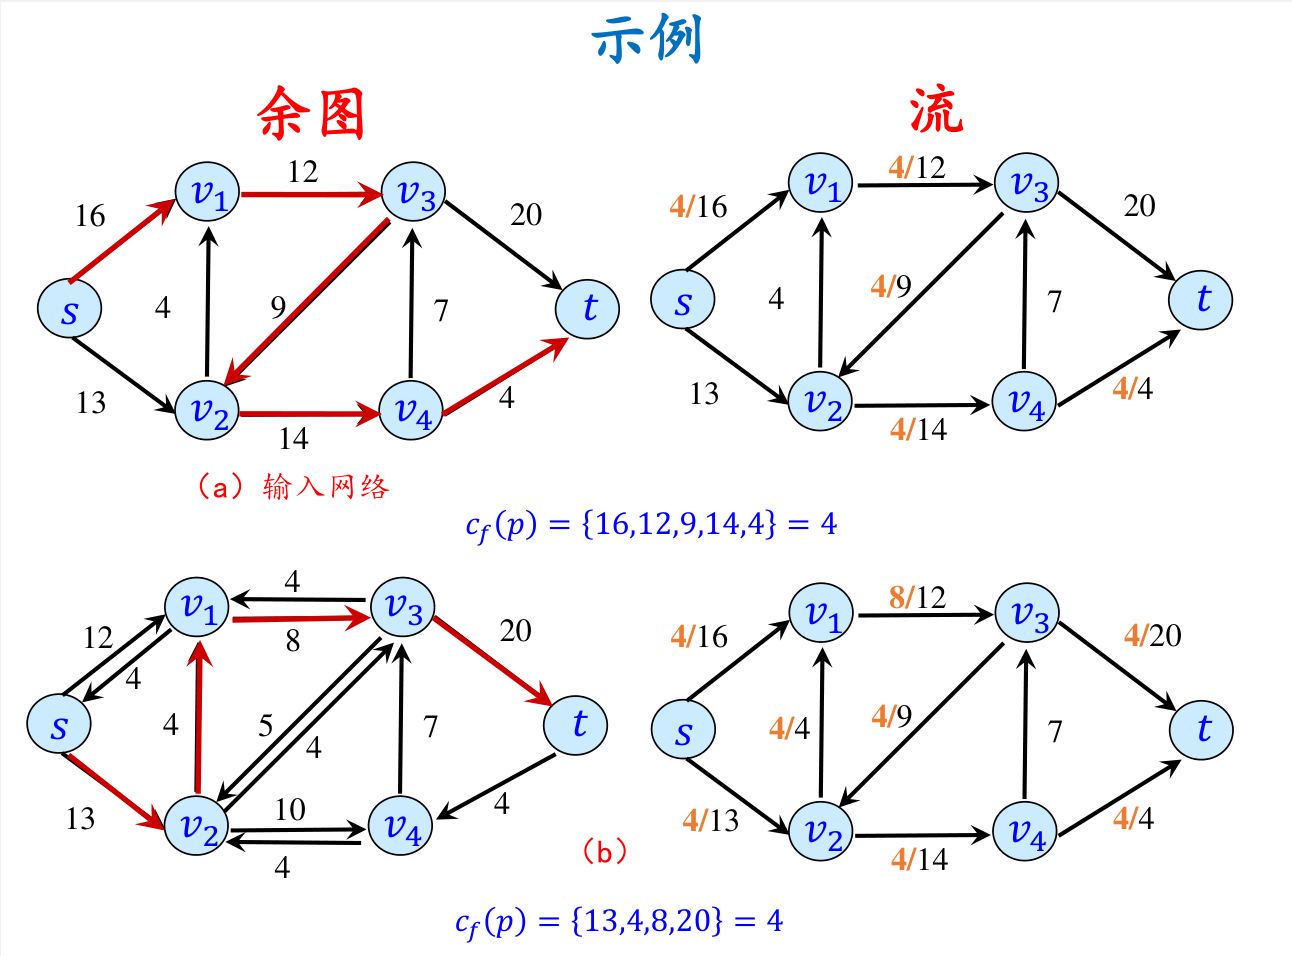
\includegraphics[scale =0.5]{mf1.png}
    \caption{实例}
    \label{fig:2}
\end{figure}
\begin{description}
    \item[1] 先是, 对于原图, 我们找到一个路径 $p$ (随便一个路径就行), 定义其 $c_{f} \left(p\right) = 4$
    \item[2] 其次, 根据此路径创建子图, 其中反向边的长度为 $c_{f} \left(p\right)$, 正向边的长度为 $c \left( u , v\right) - c_{f} \left(p\right)$. 
    反向的是因为, 不能太反, 不然两个路径加起来成负数. 正向的是因为, 相加后不能超过边的容量. 
    \item[3] 重复此操作, 直到我无法找到路径. 
\end{description}

\begin{figure}[H]
    \centering
    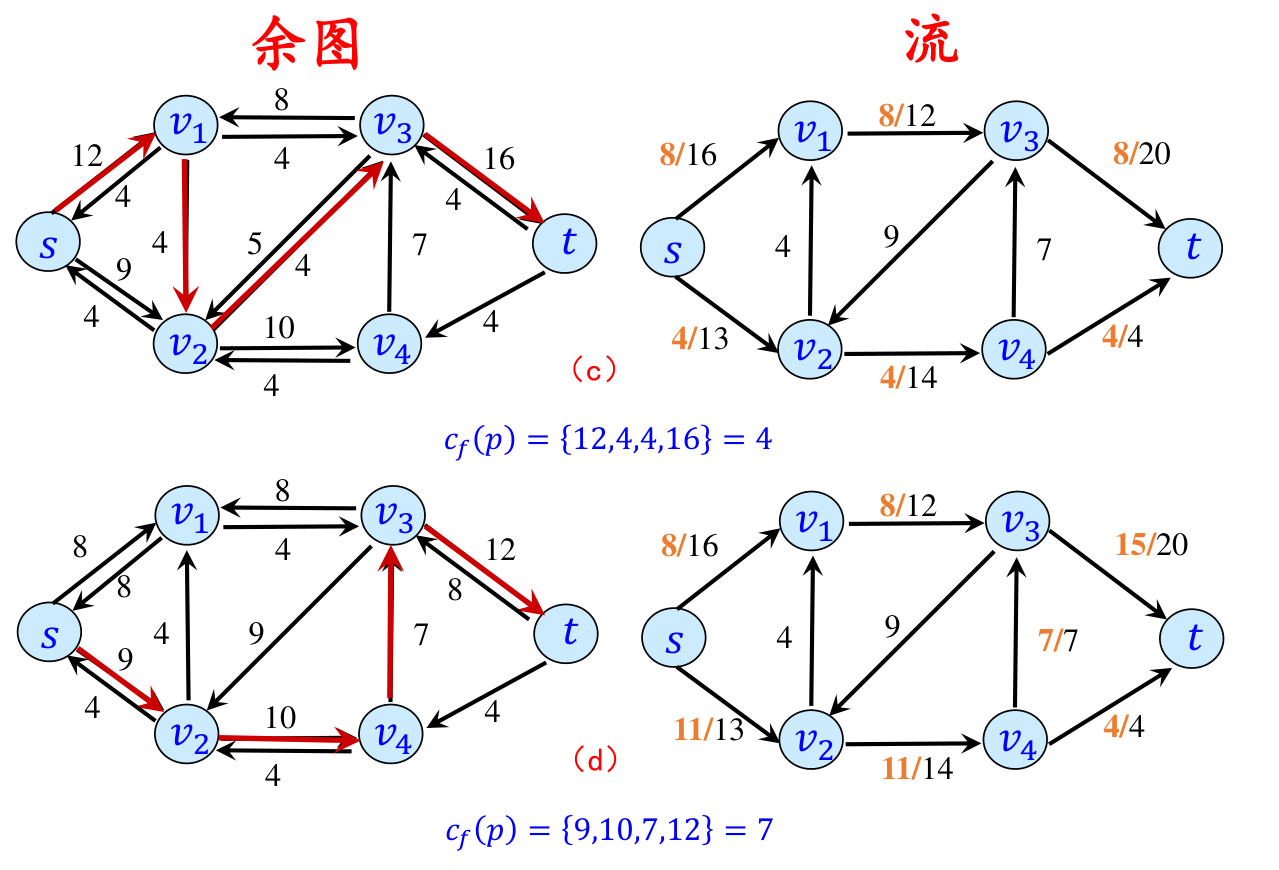
\includegraphics[scale = 0.5]{mf2.png}
    \caption{实例, 续}
    \label{fig:3}
\end{figure}
\section{method with bipartie graph}
\end{document}
